%%%%%%%%%%%%%%%%%%%%%%%%%%%%%%%%%%%%%%%%%%%%%%%%%%%%%%%%%%%%%%%%%%%
% Universidad Tecnológica de Pereira
% Facultad de Ingenierías
% Maestría en Ingeniería de Sistemas y Computación
%
% Formato para la presentación de informe final de trabajo de grado
% Versión 0.0.1 2021/10/15
%%%%%%%%%%%%%%%%%%%%%%%%%%%%%%%%%%%%%%%%%%%%%%%%%%%%%%%%%%%%%%%%%%%

\documentclass[12pt]{report}

\usepackage[utf8]{inputenc}
\usepackage[brazil]{babel}
\usepackage[letterpaper, margin=30mm]{geometry}
\usepackage{csquotes}
\usepackage{graphicx}
\usepackage{braket}
\usepackage{hyperref}
\DeclareUnicodeCharacter{0301}{\'{e}}

\usepackage[
sorting=none
]{biblatex}

\addbibresource{biblio.bib} %Imports bibliography file

\graphicspath{{Figuras/}}

\hypersetup{
    colorlinks=true,
    linkcolor=blue,
    filecolor=magenta,      
    urlcolor=cyan,
    pdftitle={mamativa},
    pdfpagemode=FullScreen,
}
    
\urlstyle{same}

\begin{document}


\newcommand{\titulo}{Documentação do Quiz para o PlacaMãe.org}
\newcommand{\nombreestudiante}{Diego Nery\\ Eduardo Henrique \\Esteffane Menezes\\ Iasmim Holanda \\Milenia Rosendo\\Rayanne Cruz \\ Ismael Mascarenhas\\ Yan Lucas \\}
\newcommand{\fecha}{\date{\today}}


\begin{titlepage}
	\centering
	
\includegraphics[width=65mm]{Figuras/unicap.png}\par
	\vspace{1cm}
	{\LARGE\bfseries \titulo \par}
	\vfill
	{\large Relatório Técnico de Conclusão de Curso da turma\\de Sistemas Para Internet\par

	\vfill
	Autores:\par\vspace{2mm}
	\nombreestudiante\par
    \vfill
    Universidade Católica de Pernambuco\par
    Sistemas para Internet \\ Data de Emissão: 07/05/2024
 \par}
\end{titlepage}

\tableofcontents
\listoffigures
% \listoftables

\chapter{Introdução}


\section{Inicio da Contextualização e Motivação}

Segundo estudos realizados em escolas de São Paulo em junho de 2020, a crescente integração da tecnologia em ambientes educacionais tem sido acompanhada por um aumento preocupante na incidência de cyberbullying. Este fenômeno, caracterizado pela prática de agressões, humilhações e ameaças por meio de dispositivos eletrônicos e redes sociais, tem impactos significativos na saúde mental e no bem-estar dos estudantes. Este documento busca fornecer uma visão abrangente sobre o cyberbullying em escolas brasileiras, com base em pesquisas realizadas em diversas regiões do país.

De acordo com os dados coletados, aproximadamente 37\% dos alunos investigados estavam envolvidos em situações de cyberbullying. Esses casos variaram desde vitimização exclusiva até participação como agressores ou vítimas-agressores. Além disso, os resultados revelaram diferenças significativas de gênero nas formas de cyberbullying experimentadas, destacando a importância de estratégias de intervenção sensíveis ao contexto.

Nesse contexto, a plataforma de Quiz desenvolvida pelo site PlacaMãe.Org surge como uma ferramenta promissora para enfrentar o cyberbullying e promover uma cultura de respeito e inclusão nas escolas.
Ao gamificar o processo de aprendizagem, a plataforma de Quiz oferece uma maneira envolvente e interativa de educar os alunos sobre a importância do respeito online e do comportamento ético nas redes sociais. Além disso, ao fornecer informações e recursos educacionais sobre o cyberbullying de forma acessível e atraente, a plataforma capacita os alunos a reconhecerem, prevenirem e denunciarem situações de violência virtual.

 

\section{Problemática}
O Bullying se encontra em relevância no cenário atual e a sua abordagem é crucial,visto que está marcado por transformações sociais e tecnológicas profundas, especialmente com o uso da internet por crianças, adolescentes e jovens, conhecidos como "nativos digitais". Essa imersão tecnológica requer uma reavaliação das estruturas sociais, desde a relação com o conhecimento até as interações interpessoais. Nesse contexto, surge como ponto central o fenômeno do cyberbullying, uma forma de violência presente no ambiente virtual com impactos significativos no bem-estar e saúde mental dos jovens.

A preocupação com o uso inadequado da internet e suas consequências negativas, como o cyberbullying, desafia o ordenamento jurídico a regulamentar essas questões de maneira eficaz. Destaca-se a importância de compreender o papel da escola, como parte da rede de proteção infantojuvenil, na prevenção e combate a essa forma de violência. A escola é considerada um espaço privilegiado para a implementação de ações educativas e preventivas, visando conscientizar os jovens sobre os riscos associados ao uso inadequado da internet e formas de prevenir o cyberbullying.

Além disso, ressalta-se a necessidade de implementação de políticas públicas e programas específicos, conforme estabelecido na Lei 13.185/2015, que criou o Programa de Combate à Intimidação Sistemática. Essa legislação representa um marco na luta contra o cyberbullying, propondo medidas preventivas e restaurativas para lidar com os conflitos. No entanto, sua eficácia depende da articulação efetiva da rede de proteção à infância e adolescência, envolvendo não apenas as escolas, mas também famílias, comunidades e órgãos governamentais.

Assim, o evento destaca a complexidade do fenômeno do cyberbullying e a necessidade urgente de uma abordagem multidisciplinar e integrada para combatê-lo. É crucial unir esforços para estabelecer um conjunto de normas que protejam efetivamente a infância e a adolescência brasileira, promovendo um ambiente seguro e inclusivo, tanto no mundo físico quanto virtual.

Em resumo, as principais questões a serem resolvidas consistem em: 
\begin{itemize}
    \item O Controle do acesso a informação disponível para os menores de idade
    \item A forma de acompanhamento dos pais com as crianças fora da escola
    \item A criação de uma legislação mais assertiva e especifica para lidar com esse tipo de caso
\end{itemize} 

\section{Objetivos}


\subsection{Objetivo Geral}

Incentivar o aumento de doações de leite materno nos bancos de leite do estado de Pernambuco.


\subsection{Objetivos Específicos}

\begin{itemize}
  \item Conscientizar nutrizes acerca da importância e dos benefícios da doação do leito materno.
  \item Disponibilizar o quantitativo dos estoques dos BLH atualizados semanalmente, para que as doadoras tenham ciência das unidades com maior necessidade e assim possam direcionar melhor sua doação.
  \item "Gameficar" a aplicação a fim de promover um maior engajamento por parte dos usuários.
\end{itemize}


 
\chapter{Trabalhos Relacionados}

Algumas iniciativas similares foram identificadas no campo de estudo deste trabalho, as quais serão apresentadas a seguir. Estas poderão ser utilizadas como referências importantes para aprimoramento e desenvolvimento da nossa aplicação.\\
\begin{enumerate}
    \item O aplicativo de celular \emph{Amamenta Brasília}, disponível para Android e IOS, funciona desde 2017. Criado pela Secretaria de Saúde do Distrito Federal, o app tem o objetivo de incentivar e apoiar a amamentação. Funciona fornecendo informações sobre aleitamento materno, materiais educativos e informações sobre bancos de leite. Uma funcionalidade importante do site é a possibilidade de agendamento para a coleta em domicílio do leite humano ordenhado pelas mulheres que desejam doá-lo. A busca do alimento é realizada pelo corpo de bombeiros do DF que o encaminha aos bancos de leite da região. A página do programa \cite{amamentabrasilia} traz mais informações
    \item Em 2018 foi lançado no Ceará, por  \cite{Carvalho}, o aplicativo para celular \emph{Amamente e Doe}. A aplicação propõe uma solução semelhante ao Amamenta Brasília, porém, sem envolvimento do estado. O aplicativo reunia informações sobre a importância da doação de leite, benefícios do aleitamento materno e auxiliava no processo da coleta de LH e armazenamento do mesmo. Bem como orientava como proceder para efetivar a doação e identificava a localização dos postos de coleta e bancos de leite humano (BLHs) do estado. Infelizmente, por motivos desconhecidos, o aplicativo não encontra-se mais em funcionamento.
    \item No ano de 2022, o então deputado Francisco Jr (PSD-GO), apresentou à câmara o Projeto de Lei(PL) 870/22 o qual instituía a criação de um Banco Virtual de Leite Materno. A ideia era desenvolver um aplicativo para dispositivos móveis para permitir que as doadoras de leite humano tivessem acesso ao sistema de gerenciamento dos bancos de leite da rede pública de seu estado As usuárias poderiam agendar através do app a retirada do leite já ordenhado pelo agente público responsável pela coleta domiciliar, além de ter acesso a informações sobre os procedimentos para adequada coleta e conservação do leite. O PL \cite{PL870/2022} atualmente aguarda tramitação no senado.
\end{enumerate}

Nossa proposta de aplicação, por sua vez, se concentrará em além de trazer toda gama de informações já citadas nas plataformas acima, desenvolver uma solução tecnológica"\textit{gameficada}", a fim de deixar a experiência da doação de leite humano mais interessante.





\chapter{Metodologia}
\section{Detalhes Técnicos}
\label{sec:tech}

A nossa aplicação foi criada a caráter informativo, com textos e elementos visuais atrativos, onde foi desenvolvida inteiramente utilizando frameworks Next.js. Logo, por ser uma interface com estruturas lógicas, não possui a nescessidade da construção de uma configuração de back-end, visto que não haverá nenhum dado externo armazenado. Portanto, o usuário poderá navegar pela plataforma sem precisar fazer cadastro, login ou fazer a inserção de qualquer outro tipo de dado.

\subsection{Front-End}
O Front-end é implementado em \cite{Next.Js} como mostra a Figura \ref{fig:logicFront}

\begin{figure}[h!]
    \centering
    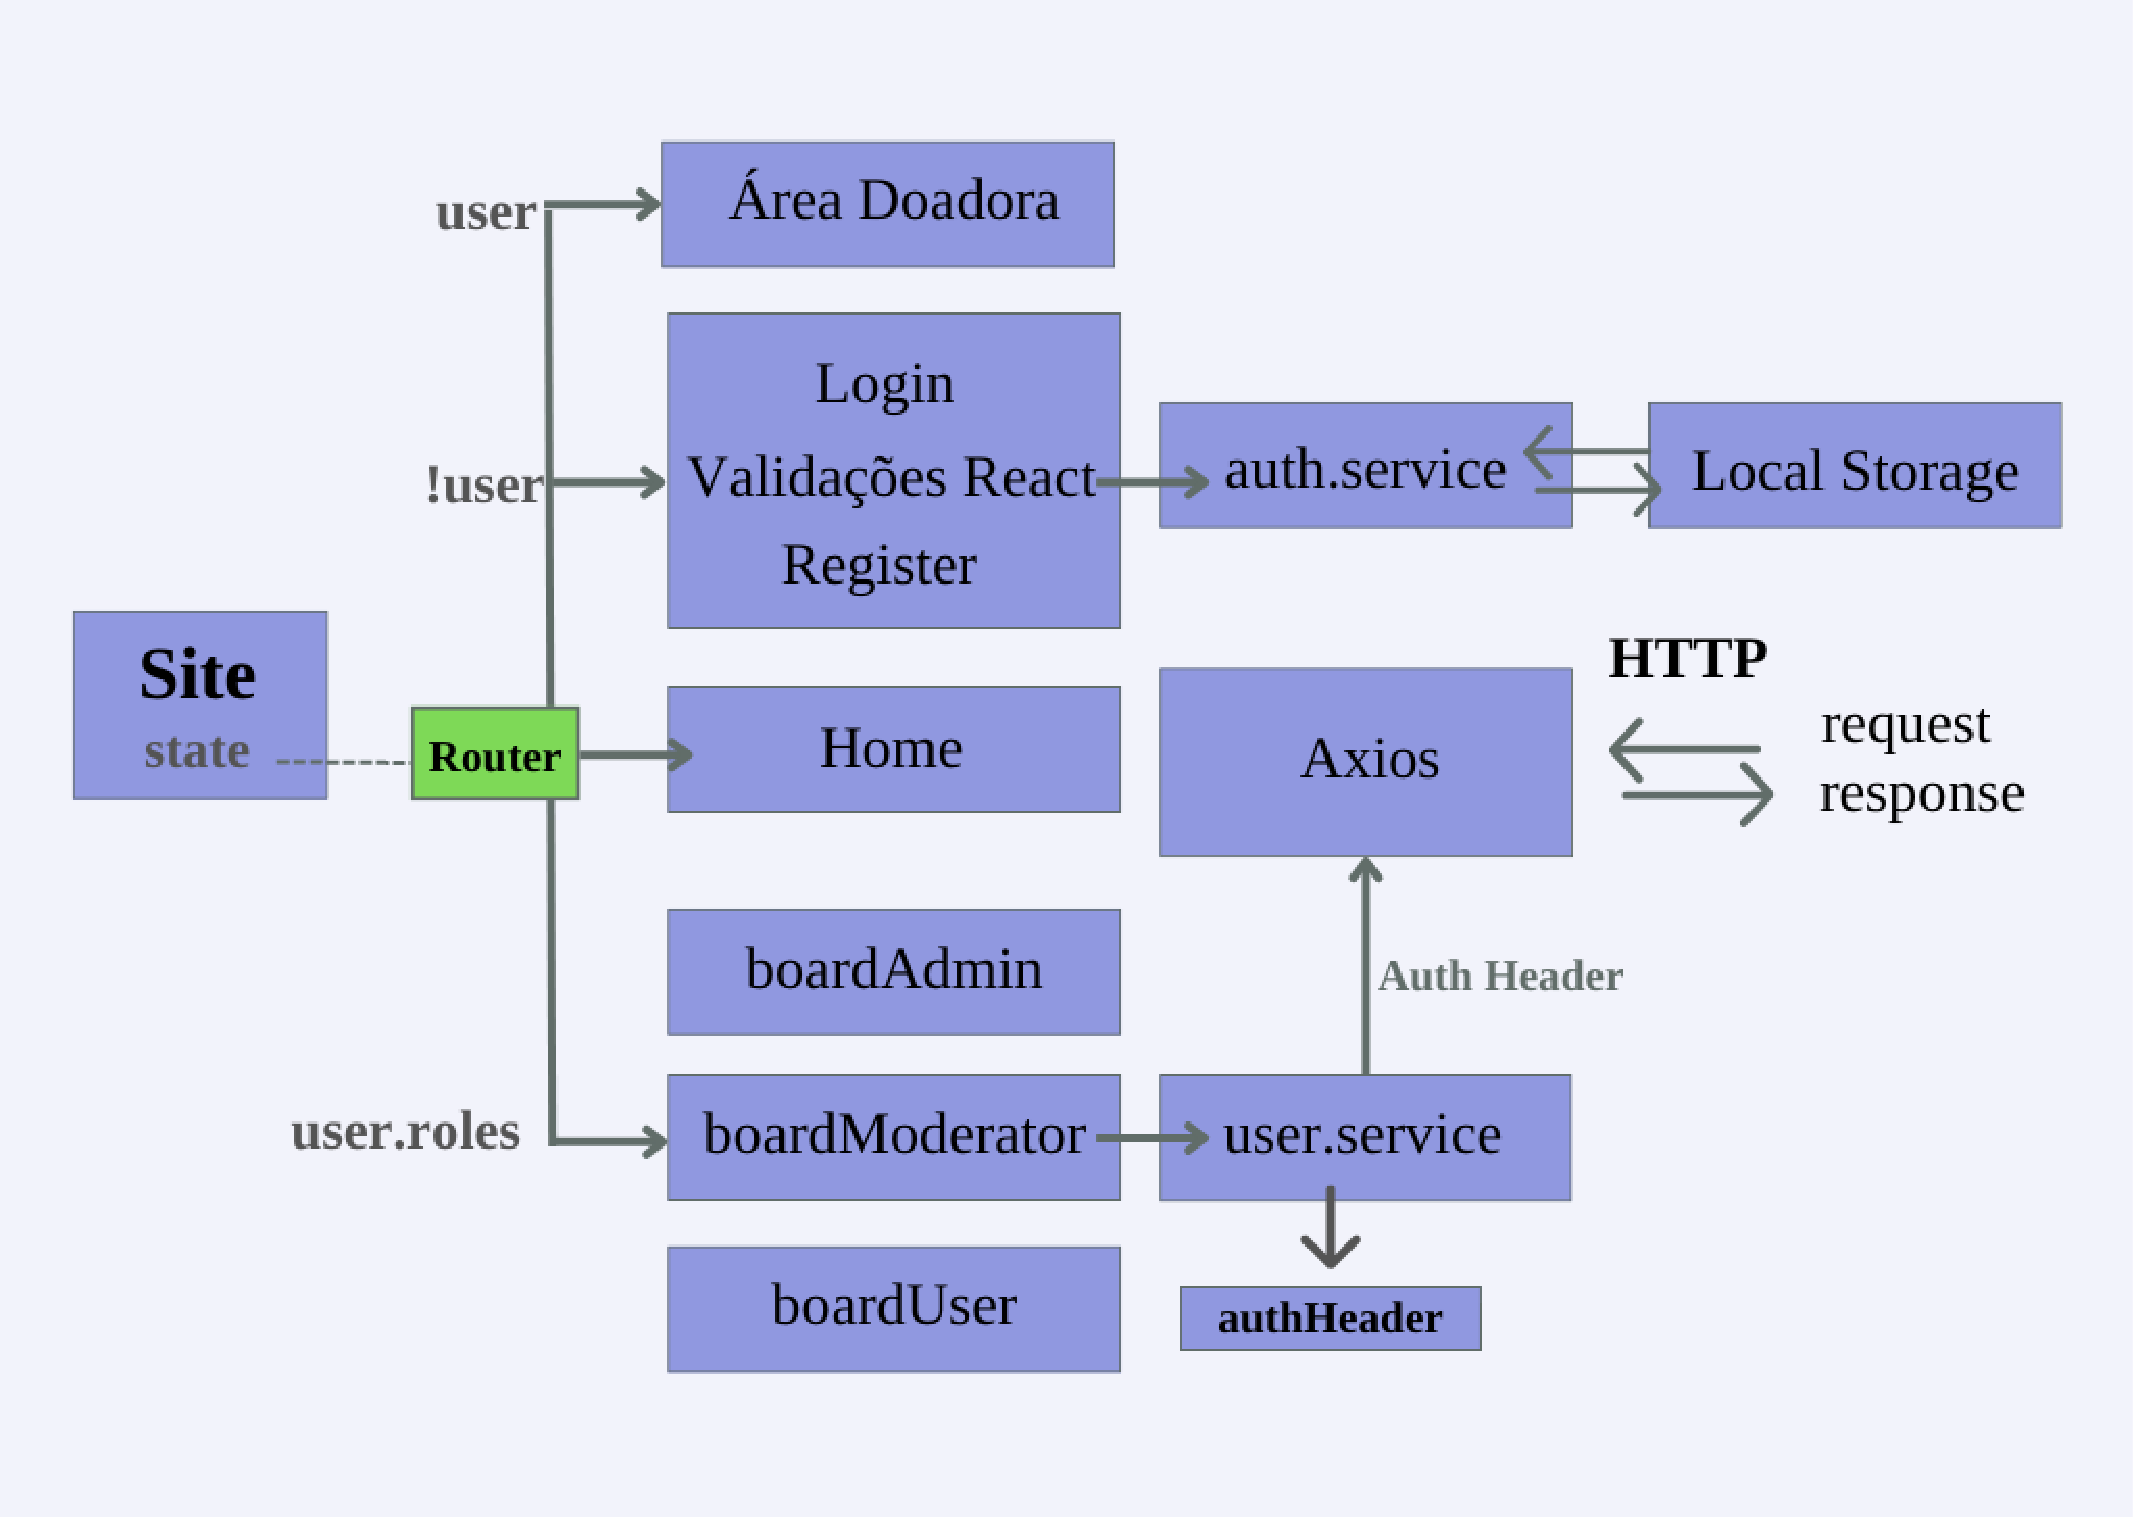
\includegraphics[width=1.0\textwidth]{Figuras/Frontpdf.pdf}
    \caption{Estrutura lógica do Front-End composta por React}
    \label{fig:logicFront}
\end{figure}

A plataforma apresenta uma tela inicial onde exibe o material de apoio para introduzir o conteúdo para estudo e aprendizado. Nesta tela também é apresentado um botão de denuncia, de extrema importância para o acionamento imediato do suporte nescessário par a situação. E a área também dispões de uma barra de navegação lateral que aponta os componentes a seguir:

\begin{itemize}

    \item Área do questionário, onde o usuário vai poder fazer a interação gameficada baseado no conteúdo apresentado na plataforma. O quiz apresenta três níveis: fácil, médio e dificil, desta forma o usuário irá fixar melhor o conteúdo apresentado na plataforma. 
 
    \item  Área de certificação, após a conclusão do quiz, o usuário poderá receber o certificado de acordo com a quantidade de acertos. Para receber o certificado o aluno precisa acertar mais de 7 questões. Criamos um algoritmo de verificação onde foram setadas as dificuldades em uma variável, em seguida adiocionamos uma codição no código que análisa a quantidade de acertos no quiz. 
    Caso o usuário não atinja a pontuação necessária, ele será direcionado para uma página onde será dado a opção de poder tentar realizar o quiz novamente. 
    
    \item Na área de indicações e materiais de estudo o usuário vai encontrar links de podcasts, sites, documentos literários e alguns materiais de estudo para o aprofundamento no conteúdo.
    
    \item Área de saiba mais que faz uma apresentação um pouco mais profunda de todo o contexto trazendo um pouco da história da empresa Placamãe.org, surgimento, trajetório e quais os impactos dentro da sociedade.
   
\end{itemize}

\clearpage

\subsubsection{Back-End}
Nossa plataforma tem caráter informativo, então, não se faz nescessário utilizar um sistema back-end pois não existe tráfego de dados. 

\begin{itemize}
 
\end{itemize}

\chapter{Requisitos funcionais e não funcionais}
\section{Requisitos Funcionais:}
\begin{itemize}
  \item O site permite a navegação entre as seções mencionadas no menu.
  \item  Os quizzes são divididos em categorias de dificuldade (fácil, média e difícil).
  \item O site fornece materiais de estudo relacionados aos quizzes.
   \item Home é o componente público de acesso a todos os usuários.
   \item Há uma funcionalidade de denúncia acessível em todo o site.
   \item O site exibe recomendações de livros, podcasts e artigos científicos sobre ciberbullying.
   \item  Links para redes sociais são funcionais onde direcionam para as páginas corretas.
\item Há um e-mail de contato visível em todo o site.
\item Informações sobre consultoria, palestras e cursos estão disponíveis.
\end{itemize}

\label{sec:tech}


\subsection{Requisitos Não Funcionais:}
\begin{itemize}
\item O site é seguro, utilizando protocolos HTTPS.
\item O site é acessível, seguindo as diretrizes WCAG. 
\item O site está esponsivo para dispositivos móveis e que suas fontes de informações são verificadas e de uso comprovado academicamente
\end{itemize}
\clearpage

\section{Descrição Geral}
\label{sec:descricao}
Para o projeto final, foi proposto o desafio de desenvolver um site interativo, enriquecido com um jogo, com o objetivo de ser educativo, envolvente e um canal para denúncias. Este site tem como meta auxiliar professores, alunos e famílias a compreenderem e combaterem o cyberbullying, alertando sobre os riscos e as ações que podem levar a incidentes de bullying. \\

O cyberbullying é um problema crescente na era digital, com consequências potencialmente devastadoras para os indivíduos afetados. Através deste projeto, espera-se fornecer uma ferramenta valiosa para combater este problema, educando e informando os usuários sobre o cyberbullying e fornecendo um meio seguro e anônimo para denunciar incidentes de bullying.\\

Este projeto está alinhado à Agenda 2030 da ONU, que estabelece 16 Objetivos de Desenvolvimento Sustentável (ODS). Em particular, o projeto se concentra no ODS 3, que é voltado para a saúde e o bem-estar. Este objetivo enfatiza a importância de garantir vidas saudáveis e promover o bem-estar para todos, em todas as idades. Ao combater o cyberbullying, este projeto contribui para este objetivo, ajudando a criar um ambiente online mais seguro e saudável para todos.\\

A plataforma foi projetada para facilitar todos os passos que envolvem esse processo, além de oferecer funcionalidades que visam incentivar o engajamento de novos indivíduos na luta contra o cyberbullying. A plataforma online será dividida em quatro seções principais, cada uma com suas próprias funcionalidades, que serão descritas a seguir.

\begin{itemize}
    \item A seção "Questionário" apresentará perguntas de níveis fácil, médio e difícil sobre o tema, baseadas em ebooks, podcasts e artigos científicos. Esta seção também incluirá exemplos práticos de situações de cyberbullying no dia a dia, com um total de 13 questões para cada nível. O objetivo desta seção é testar o conhecimento do usuário sobre o tema.

    \item A seção "Indicações/Materiais de Estudo" disponibilizará ebooks gratuitos fornecidos pelo placamae.org, podcasts recomendados por especialistas no assunto, bem como artigos científicos para auxiliar nos estudos e pesquisas relacionadas ao tema. Esta seção é uma rica fonte de informações e recursos que os usuários podem usar para aprofundar seu conhecimento sobre o cyberbullying.
    \item A seção "Saiba Mais" fornecerá informações detalhadas sobre a história do placamae,esta seção oferece uma visão abrangente sobre esta organização que busca conscientizar a todos nos meios digitais. É uma oportunidade para os usuários aprenderem mais sobre a organização por trás desta iniciativa e seu compromisso com a promoção de um ambiente online seguro

\end{itemize}

Como pode ser observado, a plataforma funcionará como um facilitador entre professores, alunos e famílias, com o objetivo de auxiliar no combate a um problema tão relevante como o cyberbullying, não só em uma cidade específica, mas em todo o país e até mesmo globalmente. Este projeto representa um esforço significativo para usar a tecnologia como uma força para o bem, fornecendo aos usuários as ferramentas e informações necessárias para combater o cyberbullying. A expectativa é que esta plataforma possa ter um impacto positivo na vida dos usuários e na comunidade online como um todo, contribuindo para um ambiente digital mais seguro e inclusivo.


\chapter{Funcionalidades e Casos de Uso}
\section{Descrição Geral}
\label{sec:descricao}
Esta plataforma está sendo desenvolvida, como extensão informativa de uma empresa com foco social, denominada PlacaMãe.Org, onde disopnibiliza de conteúdo de qualidade e de utilidade pública, sendo todos de autoria dos colaboradores envolvidos, onde existe a participação e construção saudável de uma cultura de proteção de dados pessoais em prol de um cidadania digital de excelência.
Com isso, visando contribuir positivamento com esta comunidade, surge a ideia de elaboração de uma plataforma para explanar sobre um tema em crescimento e pouco falado, que é o cyberbulling, com o objetivo de informar, orientae e auxiliar pessoas na prevenção e conhecimento sobre o assunto.


Tivemos como motivação para iniciar o nosso projeto a agenda 2030 da ONU, que aborda 16 objetivos de desenvolvimento sustentável(ODS). Nos baseamos em específico na ODS 3, que trata sobre saúde e bem estar e, na meta 3.2 que
a partir da problemática, propomos a criação de uma solução tecnológica que visa incentivar a doação de leite materno bem como trazer informações relevantes a potenciais doadoras, além de potencializar as ações já implementadas pelo governo.
Com a ideia de incentivar a nutriz a fazer a doação, facilitar esse processo é essencial. Por isso, nossa ferramente atuará de forma a facilitar todos os passos que envolvem esse processo, além de disponibilizar funcionalidades que visam prospectar o engajamento de novas doadoras. 
Nossa plataforma online contará com cinco seções, que terão suas funcionalidades descritas a seguir. 

\begin{itemize}
    \item A seção "Como Doar" trará informações, fornecidas de maneira simples e ilustrativa, sobre os procedimentos corretos e necessários para a doação de leite (apresentar números e fontes sobre leite perdido nesse processo). Será disponibilizado um passo a passo desde a ordenha até o armazenamento do alimento. Além de indicar os critérios que tornam a nutriz apta a se tornar uma doadora.
    \item A seção "Bancos de Leite" proverá informações sobre todos os bancos de leite e postos de coleta da região metropolitana do Recife, a fim de que facilitar a escolha da nutriz, seja qual for o seu critério: unidade mais próxima a sua casa, BLH com o estoque mais baixo ou mesmo unidade que tenha a opção de buscar sua doação em loco. Todas essas informações estarão visíveis para a usuária, que dessa forma espere-se que a mesma se sinta mais motivada a doar e dessa forma ajude a melhorar o quantitativo de leite nos estoques dos bancos.
    \item Na seção "Meus Registros" a nutriz terá a possibilidade de adicionar a data e a quantidade de leite doado, assim como a unidade para qual doou. Trata-se, a princípio, de uma funcionalidade que visa facilitar o controle próprio das doações que a usuária vem realizando.
    \item A seção "Mama Mídia" disponibilizará \textit{cards} informativos e descontraídos acerca da temática abordada, que estarão liberados para compartilhamento em redes sociais a fim de engajar outras potenciais doadoras ativando um gatilho social nestas, incentivando-as a conhecer nosso site e juntar-se a essa causa. Além de fazer com que a mulher que já doa sinta orgulho do seu gesto. Esta ação, também gerará pontos que acumulados poderão, a princípio, liberar insígnias e \textit{cards} especiais para a usuária em questão. Que poderão ser também compartilhados e vistos na seção que será descrita a seguir.
    \item Na seção "Minhas Conquistas" a usuária poderá visualizar seu histórico de conquistas, recompensas e liberação de selos e insígnias especiais.
\end{itemize}

%coloca dados na metodologia para acrescentar no texto em mostra visibilidade.

Como pôde ser percebido, nossa plataforma funcionará como facilitadora entre a nutriz e os BLHs, a fim de suprir essa demanda tão relevante em nossa cidade. 

\begin{figure}[h!]
    \centering
    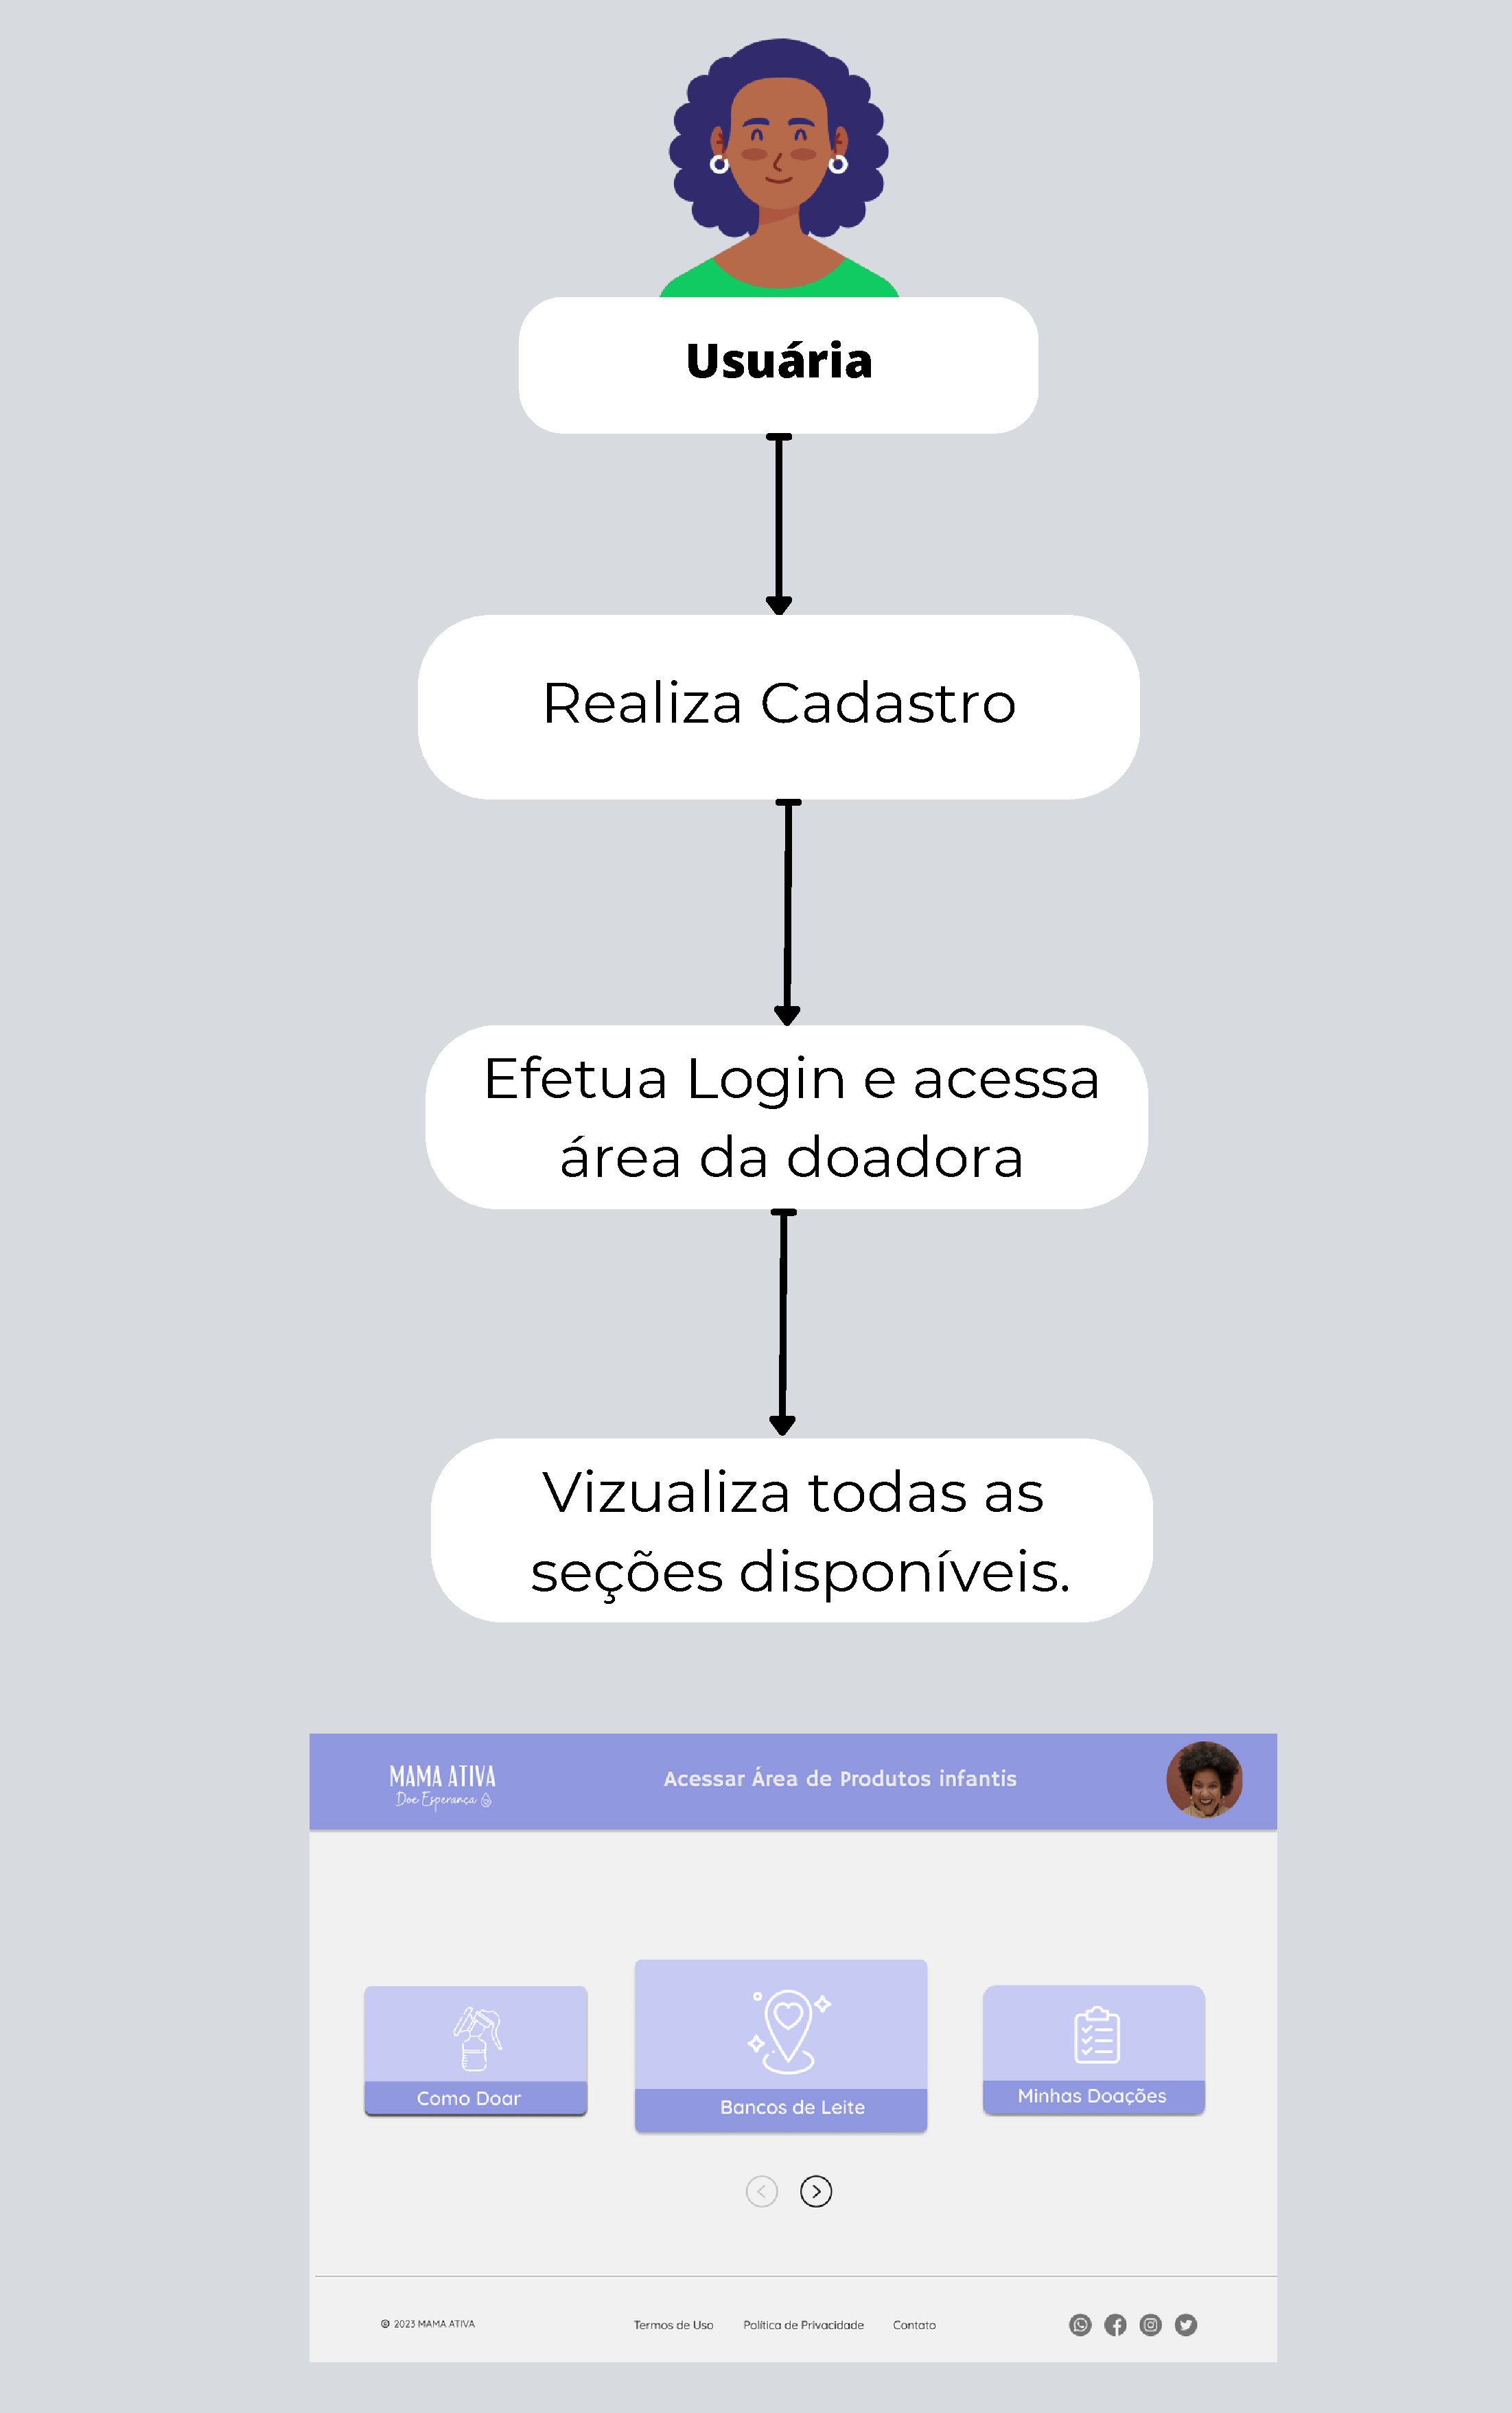
\includegraphics[width=0.45\textwidth]{Figuras/cs1.pdf}
    \caption{Caso de Uso 1}
    \label{fig:cs1}
\end{figure} 

\section{Possíveis Casos de Uso}

\begin{figure}[h!]
    \centering
    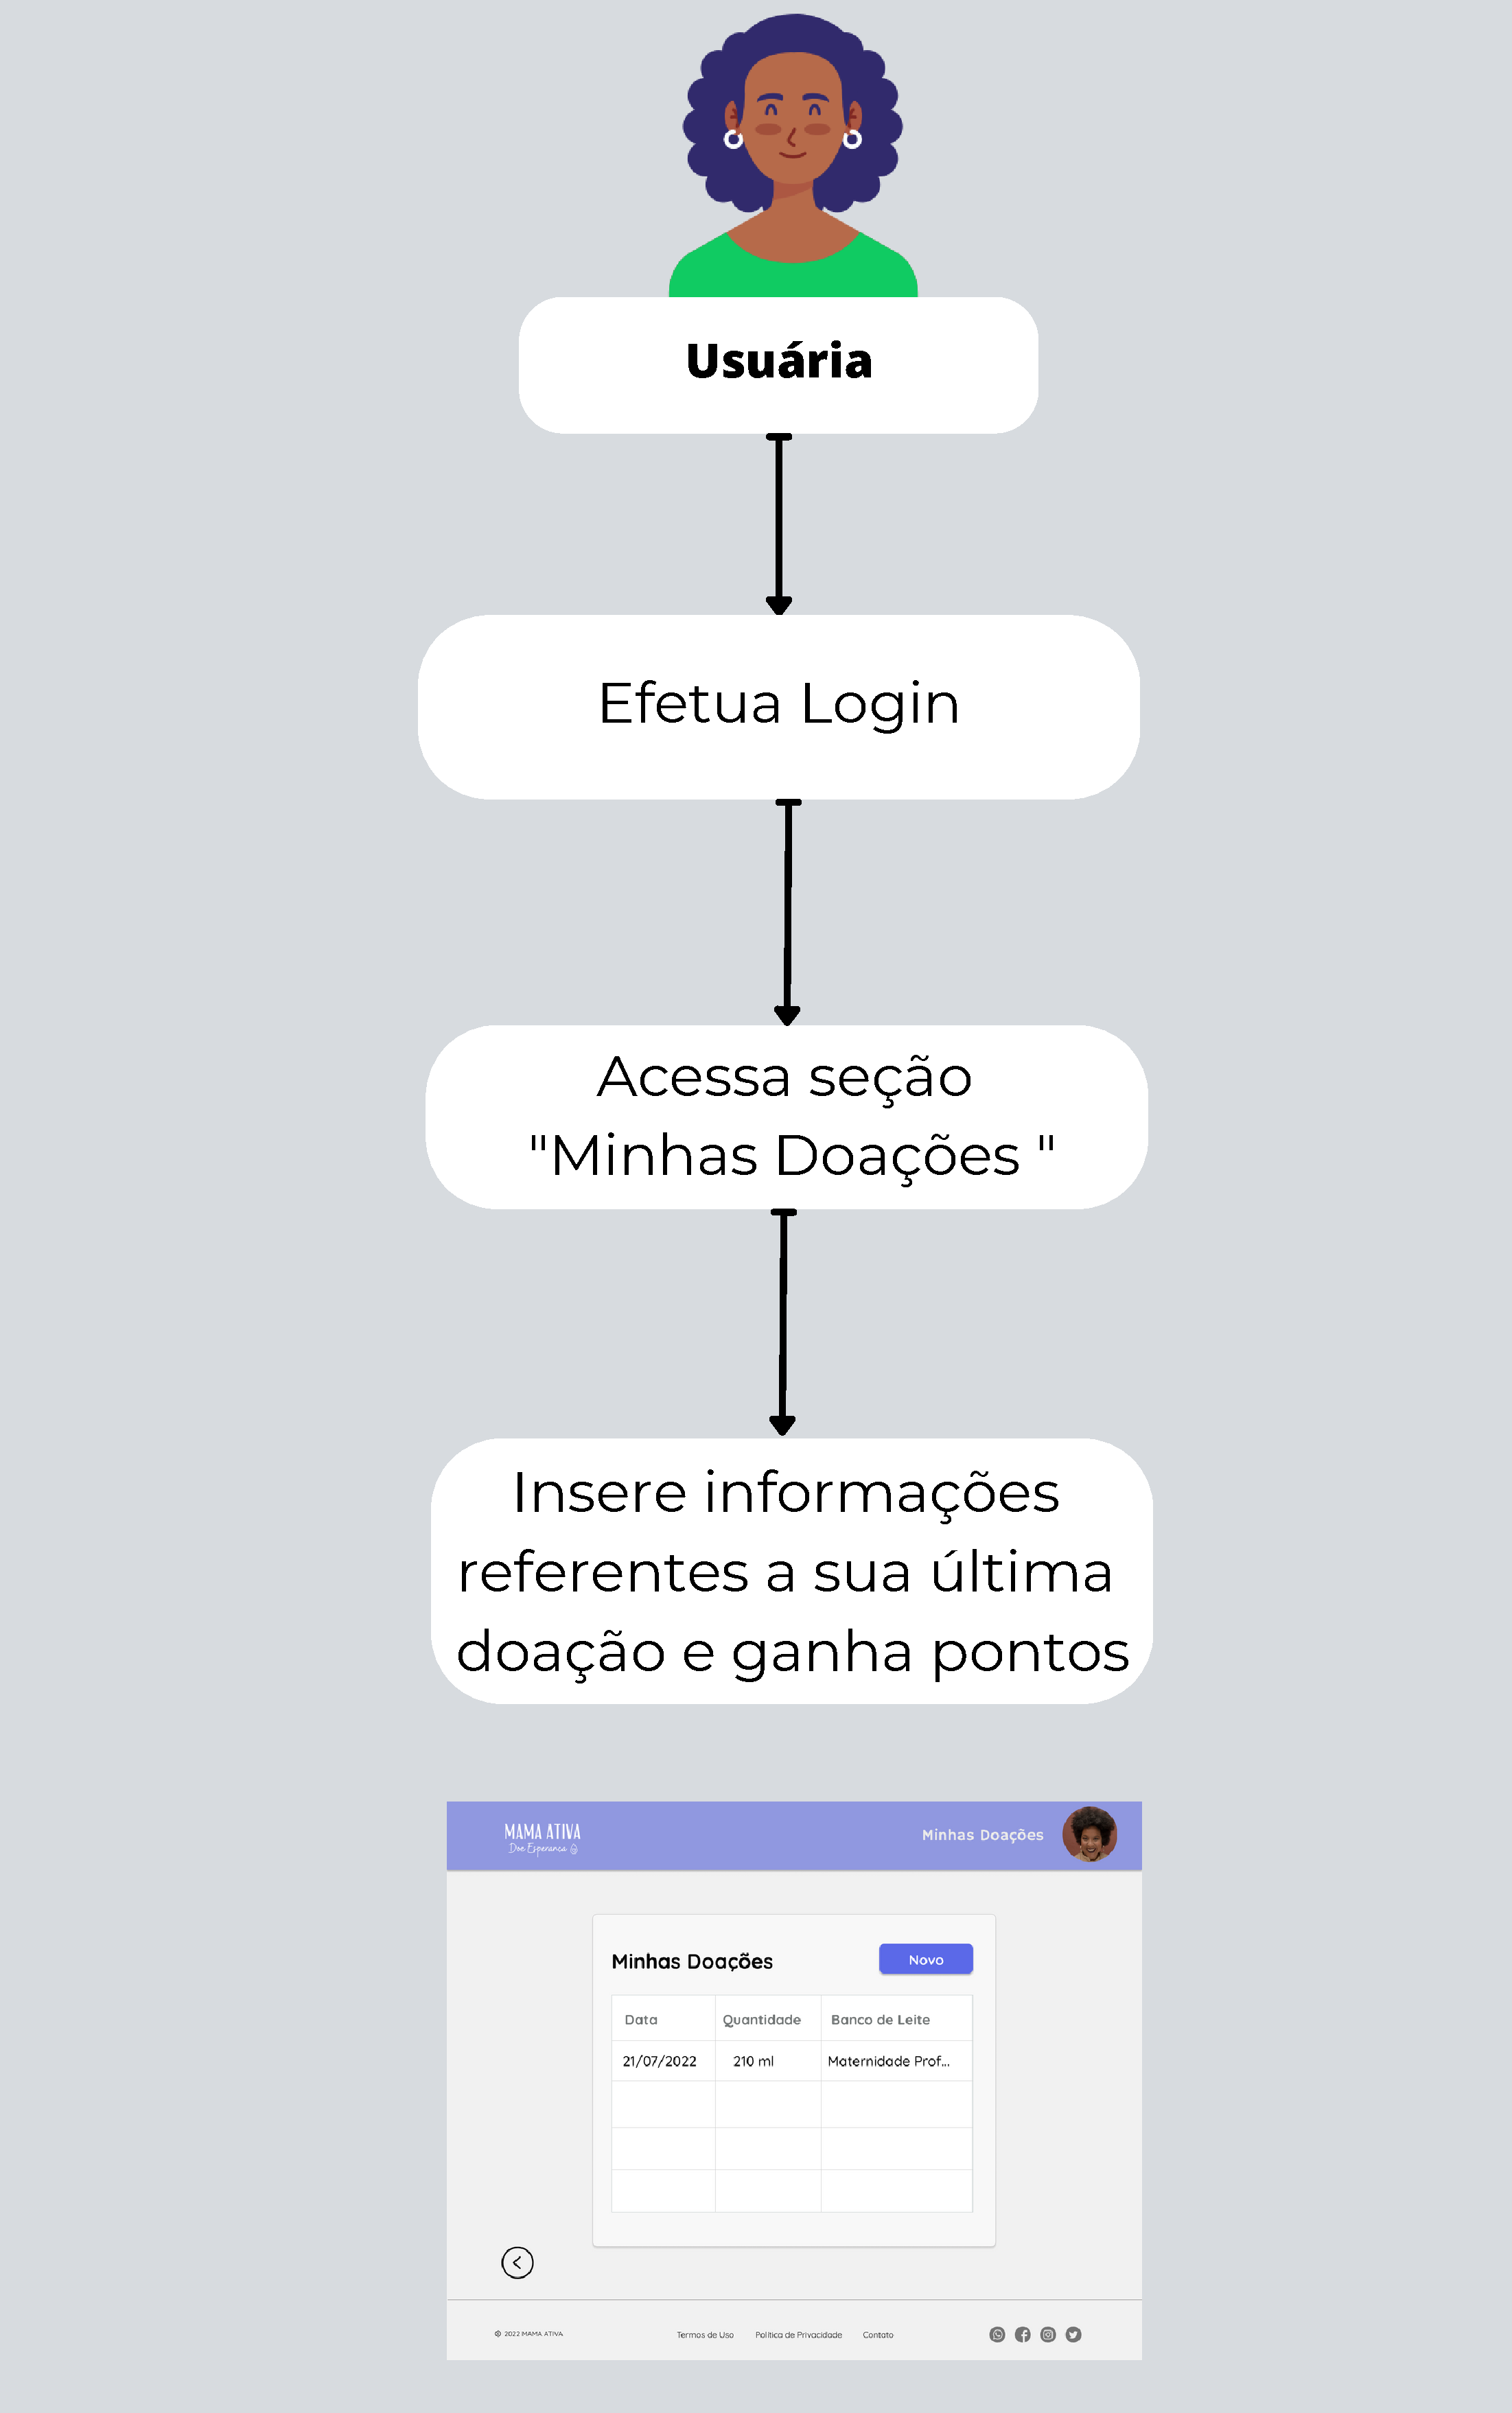
\includegraphics[width=0.45\textwidth]{Figuras/cs2.pdf}
    \caption{Caso de Uso 2}
    \label{fig:cs2}
\end{figure}

\subsection{Caso de Uso 1}
Objetivo da usuária: Realizar Cadastro e conseguir acessar área da doadora para então visualizar as seções disponíveis.

Como apresentado na Figura \ref{fig:cs1} Após o processo de cadastro, a usuária poderá fazer o login na página inicial e então poderá acessar a área da doadora. Com o intuito de facilitar a experiência de se tornar doadora, essa parte da ferramenta irá expor de forma simples e direta todas as seções disponíveis: Como doar, Bancos de Leite, Meus Registros, Mama Mídia e Minhas Conquistas. 

\subsection{Caso de Uso 2}
Objetivo da usuária: Acessar site e inserir em seção com este fim, informações referentes a sua última doação de leite.

Como apresentado na Figura \ref{fig:cs2}, ao efetuar o login, uma das seções que a usuária terá acesso é “Minhas Doações”. Aqui, a doadora poderá registrar informações relacionadas a sua última doação, como a data e a quantidade de leite doado e a unidade para qual doou. Com os dados inseridos, o aplicativo então irá fornecer pontos de acordo com a quantidade de leite doado.

\subsection{Caso de Uso 3}
Objetivo da usuária: Acessar site e a partir de seção que lista todos os Bancos de leite da cidade, encontrar o que fica mais próximo a sua casa.

Após o processo de login, a usuária poderá conferir informações sobre os bancos de leite da região metropolitana do Recife através da seção “Bancos de Leite”, como apresentado na Figura \ref{fig:cs3}. A nutriz poderá utilizar a ferramenta de busca para filtrar os bancos de acordo com o bairro e encontrar o mais próximo de sua moradia. Com o banco selecionado, é possível conferir todas as informações a respeito do local.
\begin{figure}[h]
    \centering
    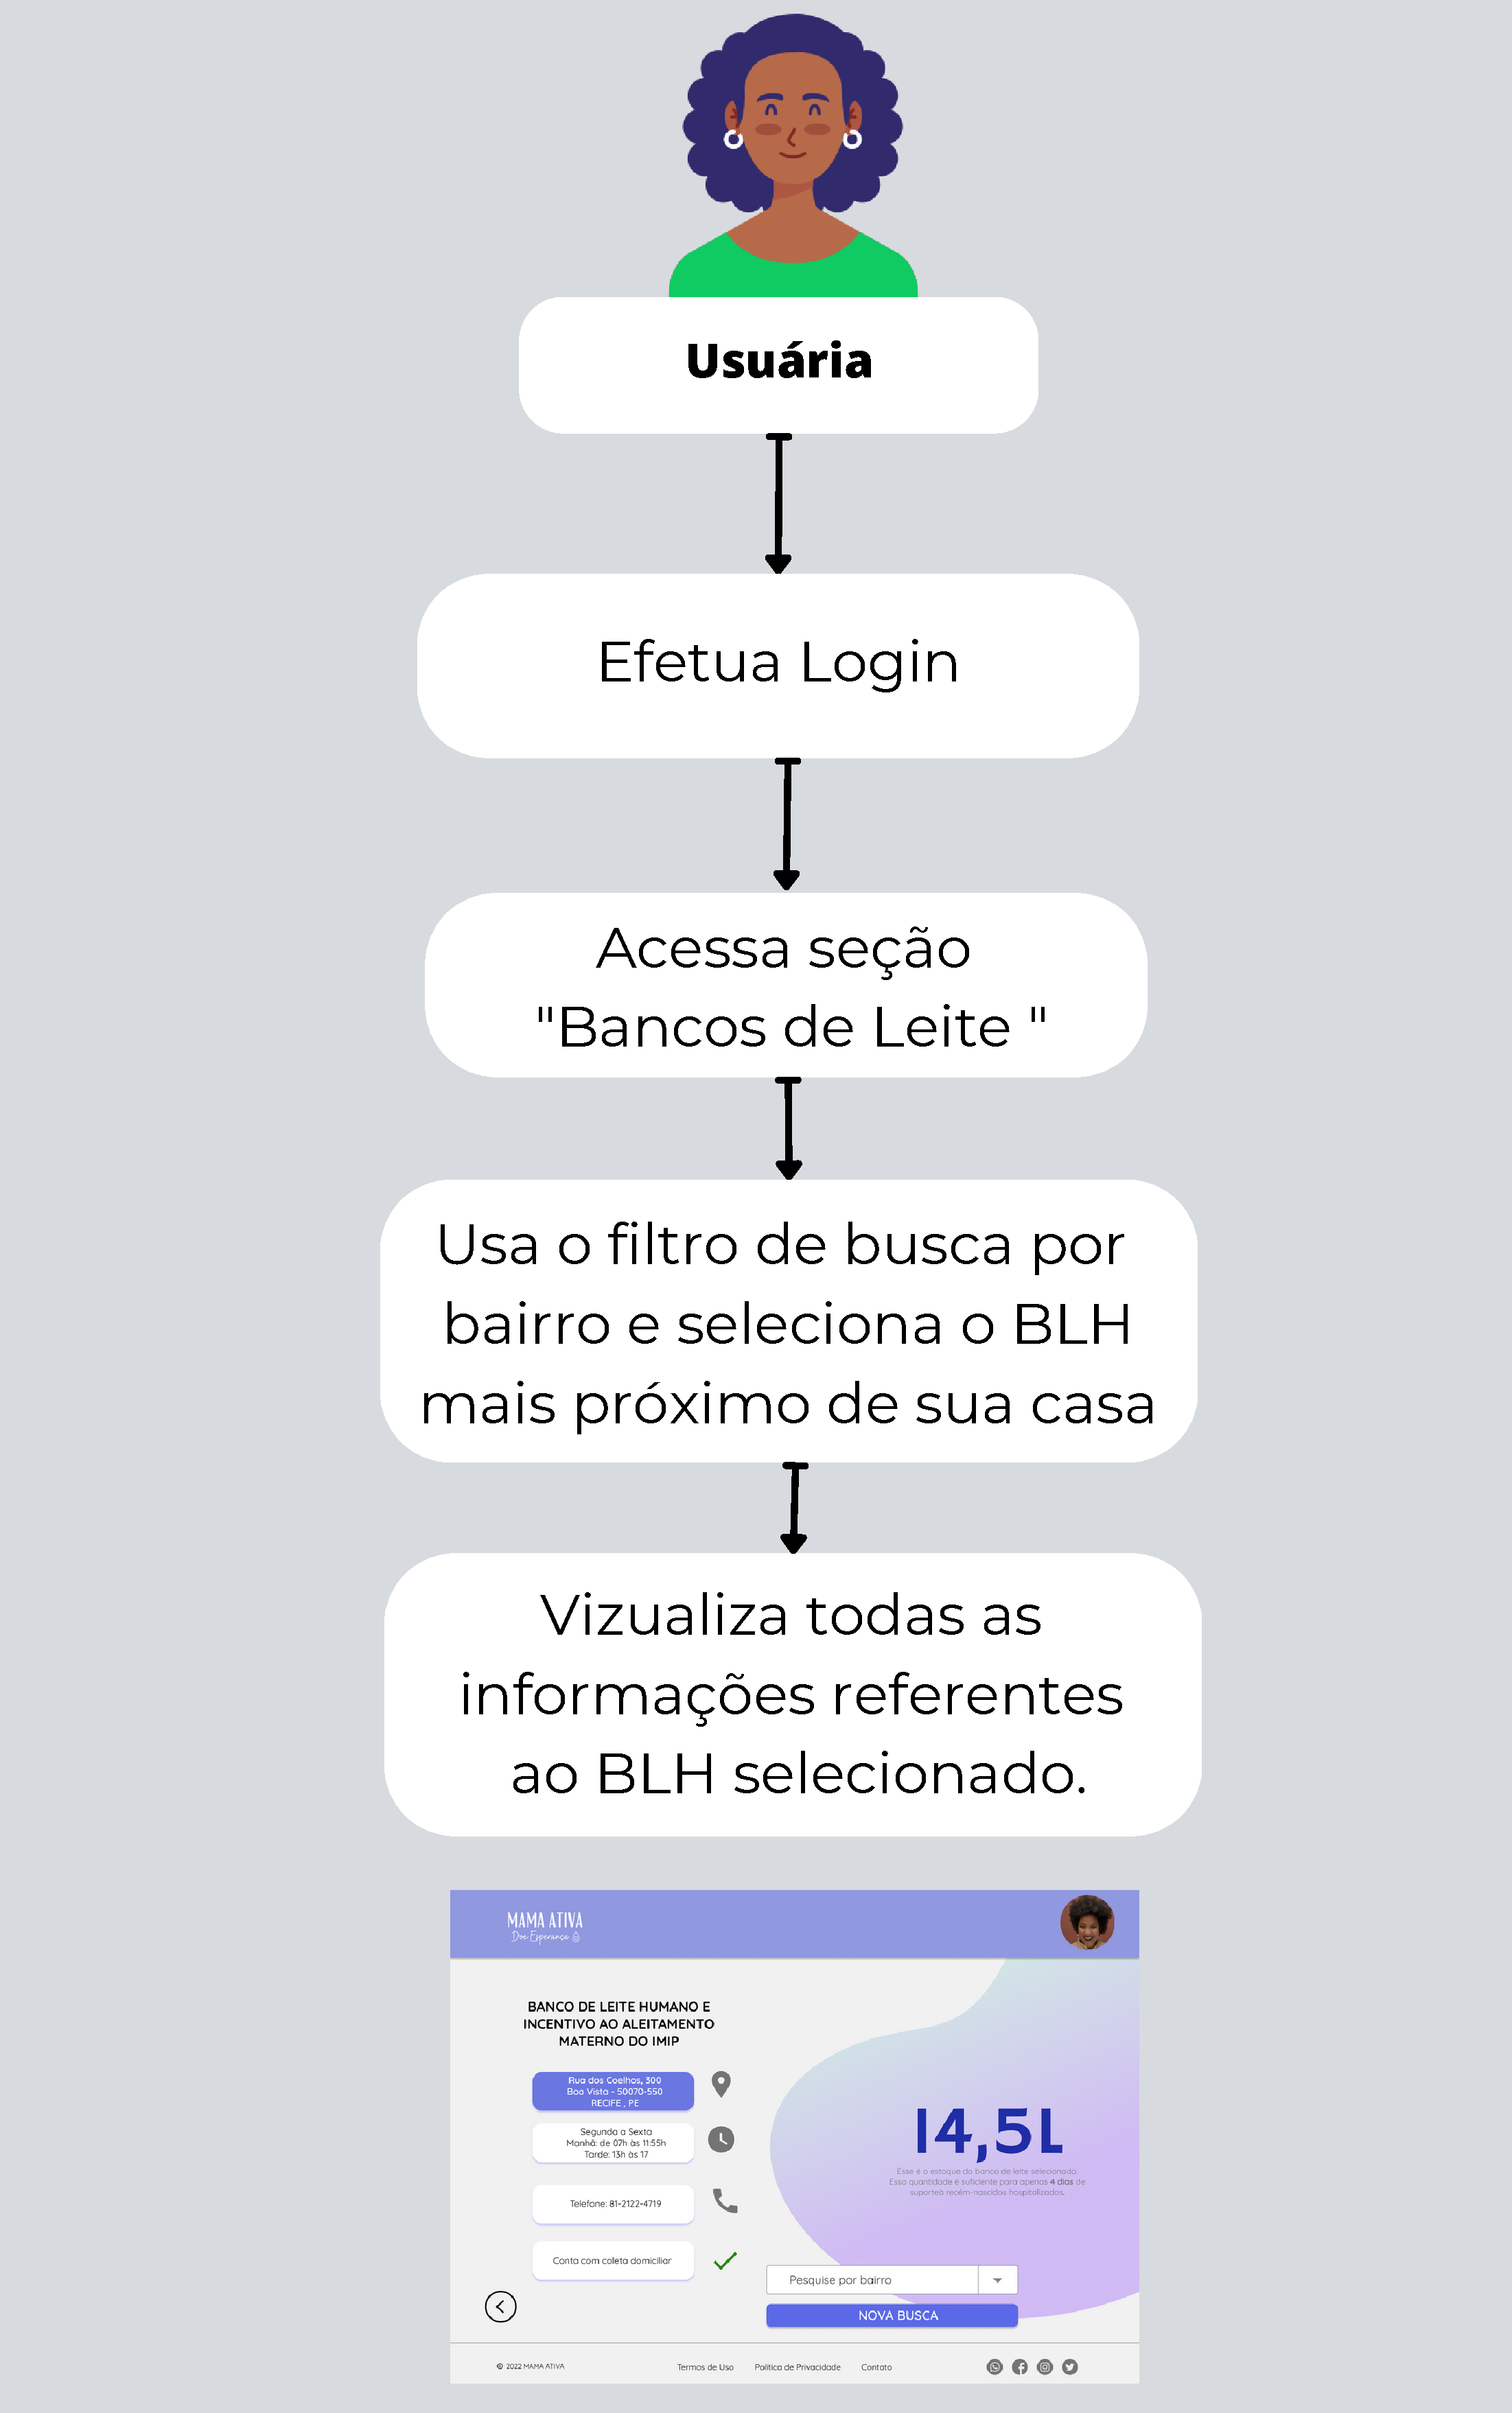
\includegraphics[width=0.45\textwidth]{Figuras/cs3.pdf}
    \caption{Caso de Uso 3}
    \label{fig:cs3}
\end{figure}


\chapter{Diagrama de Classes}


\section{Descrição do Diagrama}

O Brasil é considerado mundialmente modelo de referência em doação de leite materno, isso porque conta com a Rede de Bancos de Leite Humano (rBLH-BR), uma ação estratégica de promoção, proteção e apoio ao aleitamento materno. A iniciativa engloba ações como coleta, processamento e distribuição de leite humano para bebês prematuros ou de baixo peso que não podem ser alimentados pelas próprias mães. Em todo o país são 224 bancos de leite humano(BLH) e 216 postos de coleta, presentes em todos os estados do país.
Mesmo com uma rede tão ampla, a doação ainda não atende plenamente à demanda existente. Segundo matéria publica no Portal da Secretaria de Atenção a Saúde Primária e dados do ministério da saúde \cite{SAPS}, no ano de 2021, foram distribuídos 168 mil litros de leite humano, beneficiando 237 mil recém-nascidos. No entanto, essa quantidade representa apenas 55\% da necessidade real no país.

Um dos grandes obstáculos enfrentados no fluxo da doação de leite humano é o acesso a informação. Estudos apontam que a maioria das mulheres não tem o conhecimento de como doar, não sabem sobre a possibilidade do BLH buscar sua doação em sua casa e tampouco tem a dimensão do quanto seu gesto poderia impactar positivamente a vida de recém nascidos internados em unidades hospitalares. Trazer informação e conscientização para essas mulheres é parte da missão do Mama Ativa.

\section{Elementos do Diagrama}
No Brasil, cerca de 330 mil crianças nascidas a cada ano são prematuras ou têm baixo peso e precisam da doação de leite materno para sobreviver. O número representa 11 por cento do total de crianças nascidas no país, média de 3 milhões por ano.\cite{SAPS}
Atualmente, na cidade do Recife, são realizadas campanhas anuais de incentivo a amamentação. Porém, todos os anos, durante todo o ano, o problema se repete. Segundo \cite{FolhadePernambuco} os baixos estoques de determinados bancos chegaram recentemente a níveis preocupantes. Outra combinação preocupante que identificamos a partir de dados fornecidos pela \cite{RedeBLH}, foi que a situação dos estoques piora em datas festivas, como carnaval, natal e réveillon, ao mesmo tempo em que a necessidade deste alimento para os recém-nascidos internados em UTIs aumenta.
Identificado este problema e nos aprofundando mais em pesquisas sobre o tema, constatamos que não existe hoje, no Recife, nenhuma plataforma tecnológica que atenda a essa demanda. Dito isto, propomos a criação de uma aplicação que propõe, através de uma experiência atraente, divertida e "gameficada", incentivar o aumento de doações de leite humano(LH) em nosso estado.

Com o objetivo de entender melhor os fatores que estão diretamente relacionados a doação de leite humano, realizamos uma revisão de literatura acerca do tema. Analisamos 10 artigos científicos além de sites institucionais e governamentais. Foi observado que as principais razões encontradas para a doação de LH não começam no propósito da doação em si. Diversos artigos apontam que a maioria das mulheres procuraram os BLHs das suas cidades buscando orientação para a amamentação. Essas, relatam que após o primeiro contato com profissionais das unidades passam a saber da possibilidade do armazenamento e da doação do seu leite. 

Outras razões apontadas como relevantes para que a doação não aconteça seriam: falta de suporte emocional, ausência de rede de apoio, falta de conhecimento e dificuldade em encontrar informações acerca do fluxo de doação de LH.

Os BLHs possuem um controle de armazenamento sobre as doações que são recebidas e a quantidade disponível para doação. Antes do alimento ser direcionado para o consumo, ele passa por um processo de pasteurização, que consiste em aquecê-lo a uma temperatura elevada por um período determinado, com o objetivo de inativar 100\% dos microorganismos patogênicos, que são aqueles capazes de causar doenças em seres humanos, e cerca de 99,99\% da microbiota saprófita, que são microorganismos que auxiliam na decomposição de matéria orgânica morta. O problema é que, segundo \cite{RedeBLH}, nesse processo aproximadamente 30\% do leite doado é desperdiçado devido principalmente à forma inadequada de coleta e armazenamento. Muitas mães utilizam recipientes com tampas de alumínio, tornando-os inutilizáveis para doações posteriores. Além disso, é comum que o leite seja entregue contaminado por sujeira ou danificado pelo congelamento.

Em resumo, os principais problemas encontrados consistem de: 
\begin{itemize}
    \item Falta de acesso a informação
    \item Ausência de uma solução efetiva e durável no estímulo a doação de leite
\end{itemize} 

\section{Relações entre as classes}

\subsection{Notas e Observaçôes}

\begin{itemize}
  \item Conscientizar nutrizes acerca da importância e dos benefícios da doação do leito materno.
  \item Disponibilizar o quantitativo dos estoques dos BLH atualizados semanalmente, para que as doadoras tenham ciência das unidades com maior necessidade e assim possam direcionar melhor sua doação.
  \item "Gameficar" a aplicação a fim de promover um maior engajamento por parte dos usuários.
\end{itemize}






\chapter{Conclusão}

\section{Considerações Finais}
Com este trabalho buscamos explorar como o cyberbullying tem crescimento significativo entre os adolescentes e jovens e como a criação desta plataforma educativa é de extrema importância para atuar como uma ferramenta de combate a este tipo de violência. Juntamente com um material educativo dentro da plataforma online, procuramos mostrar a devida relevância de reconhecer esse tipo de violência e de como agir a partir deste tipo de acontecimeno, quais os direitos e atitudes a serem tomadas a partir disto.\\

Ao longo do processo de desenvolvimento, reconhecemos que o sucesso da plataforma depende da conscientização e da participação ativa dos usuários. Portanto, além de fornecer informações úteis e relevantes acerca dos procedimentos de como agir a partir de uma situação como esta, também deixamos a disposição um quiz de conscientização para enfatizar todas as informações que estão disponíveis na plataforma.\\


Este foi apenas o ponto de partida para dar ênfase a conscientização ao combate a este tipo de violência. É de suma importância acompanhar as interações dos usuários com a plataforma, obter feedbacks e assim conseguir alcançar resultados positivos em relação a diminuição de desinformação e até de casos de cyberbullying.\\


Por fim, acreditamos firmemente que o produto proposto tem um potencial significativo para promover mudanças reais e concretas. Ao buscar informar um número significativo de adolescentes e jovens, conscientizando-os sobre o cyberbullying, esta aplicação consegue contribuir efetivamente na redução de casos, no aumento dos índices de denuncias e na procura de ajuda, contribuindo com o aumento de informação sobre esta temática.


\printbibliography[heading=bibintoc, title={Referencias}]


\end{document}
